\documentclass[12pt]{article}

% Correção para erro \normalsfcodes no Overleaf / TeX Live 2025
% \makeatletter
% \DeclareRobustCommand{\normalsfcodes}{%
%   \sfcode`\.=3000
%   \sfcode`\?=3000
%   \sfcode`\!=3000
%   \sfcode`\:=2000
%   \sfcode`\;=1500
%   \sfcode`\,=1250
% }
% \makeatother

\usepackage{sbc-template}
\usepackage{graphicx,url}
\usepackage[utf8]{inputenc}
\usepackage[T1]{fontenc}
\usepackage[brazil]{babel}
\usepackage{booktabs}
\usepackage{tabularx}
\usepackage{array}
\usepackage{float}
\usepackage[hidelinks]{hyperref}

\sloppy

\title{Relatório Analítico de Performance e Capacity Planning\\
  CCO-DataOps: Escalonamento Vertical do Apache Druid}

\author{Gabriel Gonçalves Sampaio\inst{1}, Barbara Pimenta Caetano\inst{1}}

\address{Instituto de Engenharia de Sistemas e Tecnologia da Informação (IESTI) \\
  Universidade Federal de Itajubá (UNIFEI)\\
  Avenida BPS, 1303 -- 37500-903 -- Itajubá -- MG -- Brasil
  \email{gabrielsampaio059@gmail.com, bpimentacaetano@unifei.edu.br}
}

\begin{document}

\maketitle

\begin{abstract}
  The continuous ingestion and spatial processing of geographic data demands highly resilient infrastructure. This technical report details the capacity planning and performance evaluation of an event-driven DataOps architecture centered on Apache Druid. By subjecting the analytical engine to rigorous stress tests mimicking chaotic real-world queries—such as high-density GeoJSON geospatial joins and concurrent Table Scans—the limits of the system were established. Results demonstrated that the platform is profoundly CPU-bound, maintaining safe memory limits while processing over 3.3 million dynamic fire events in a highly compressed columnar footprint (566 MB). The findings technically substantiate the architectural decision to mitigate dimensional join bottlenecks through data denormalization upstream via Apache Spark, ensuring robust scalability for national civil defense monitoring.
\end{abstract}

\begin{resumo}
  A ingestão contínua e o processamento espacial de dados geográficos exigem uma infraestrutura altamente resiliente. Este relatório técnico detalha o planejamento de capacidade e a avaliação de performance de uma arquitetura DataOps orientada a eventos baseada no Apache Druid. Ao submeter o motor analítico a rigorosos testes de estresse que mimetizam consultas caóticas reais — como cruzamentos geoespaciais densos (GeoJSON) e varreduras concorrentes (\textit{Table Scans}) —, estabeleceram-se os limites técnicos do sistema. Os resultados demonstraram que a plataforma é estritamente limitada por processamento (\textit{CPU-bound}), mantendo limites de memória seguros enquanto processa mais de 3,3 milhões de eventos dinâmicos de incêndio em uma pegada colunar altamente compactada (566 MB). As descobertas fundamentam tecnicamente a decisão arquitetural de mitigar gargalos de cruzamento dimensional através da desnormalização prévia dos dados via Apache Spark, garantindo a escalabilidade robusta para o monitoramento nacional da defesa civil.
\end{resumo}

% Inclusão dos Capítulos Escritos Separadamente
\section{Introdução}

O monitoramento contínuo de focos de incêndio e eventos climáticos extremos exige uma infraestrutura de dados capaz de processar e analisar grandes volumes de informações geoespaciais e temporais em tempo real. O projeto CCO-DataOps foi idealizado para atender a essa demanda, integrando dados provenientes de satélites (como os focos de calor registrados pelo INPE) com dimensões estratégicas nacionais, incluindo infraestruturas de saúde (CNES), de logística e energia (ONS), e malhas territoriais complexas (Terras Indígenas e Municípios).

Para garantir a fluidez da exploração visual dessas informações em painéis interativos (através do Apache Superset), optou-se pela utilização do Apache Druid como motor principal de banco de dados analítico (OLAP). Diferente de bancos de dados relacionais tradicionais, o Apache Druid é otimizado para ingestão particionada e compressão colunar profunda, oferecendo baixa latência na resolução de consultas de agregações matemáticas e séries temporais aplicadas a Big Data.

Entretanto, a introdução de operações espaciais e cruzamentos dimensionais (\textit{Joins}) em tempo real traz desafios computacionais severos. O tráfego de matrizes de vetores GeoJSON, atrelado à necessidade de agrupamentos multidimensionais dinâmicos (os chamados \textit{Virtual Datasets}), pode saturar rapidamente os nós de processamento da arquitetura e degradar a experiência do usuário, extrapolando a janela aceitável de latência.

Diante deste cenário, este relatório técnico apresenta um estudo analítico e exaustivo de \textit{performance} e \textit{Capacity Planning} da infraestrutura do CCO-DataOps. Através de um simulador de concorrência extrema --- que submeteu o banco de dados a diversas rodadas de estresse, perfis de hardware variados e cenários de acesso concorrente --- objetiva-se mapear o teto de escalabilidade vertical do sistema, quantificar a eficiência de respostas do \textit{Cache} de memória, decifrar o \textit{footprint} de armazenamento em disco e, primariamente, justificar cientificamente todas as decisões de projeto adotadas para sustentar a plataforma.

\section{Objetivos}

\subsection{Objetivo Geral}
Avaliar a escalabilidade vertical, a \textit{performance} de processamento analítico e o consumo de infraestrutura da arquitetura CCO-DataOps --- com ênfase no motor Apache Druid --- sob condições de tráfego intensivo, a fim de garantir a responsividade em tempo real dos painéis gerenciais e operacionais.

\subsection{Objetivos Específicos}
Para atingir o objetivo principal, foram estabelecidos os seguintes propósitos complementares para a bateria de testes de estresse:

\begin{itemize}
    \item \textbf{Mapear a Matriz de Capacidade e Saturação:} Determinar o teto máximo de concorrência suportado pelo sistema (Usuários Simultâneos e Consultas por Segundo) antes da ocorrência de degradação de tempo de resposta (\textit{Timeouts}) ou falhas, variando os recursos computacionais disponíveis (perfis de CPU).
    \item \textbf{Mensurar a Eficiência do Mecanismo de Cache:} Quantificar o ganho real na latência proporcionado pelo \textit{Cache} de memória do Druid (\textit{Warm Cache} vs \textit{Cold Cache}), especialmente ao processar agregação massiva em \textit{Virtual Datasets}.
    \item \textbf{Identificar Gargalos Computacionais (Query Hotspots):} Isolar e catalogar as consultas SQL de maior custo sistêmico --- tais como cruzamentos de matrizes espaciais (Joins com polígonos JSON) --- comprovando gargalos arquiteturais.
    \item \textbf{Analisar a Pegada de Armazenamento (Storage Footprint):} Avaliar a taxa de compressão nativa de colunas e a fragmentação em disco, validando a sustentabilidade de longo prazo para a ingestão contínua de bases de Focos de Incêndio nacionais.
\end{itemize}

\section{Metodologia}

Para prover embasamento científico à arquitetura analítica do sistema CCO-DataOps, idealizou-se um simulador de concorrência caótica em Python (\texttt{run\_druid\_benchmark.py}). O objetivo da ferramenta é replicar de forma fidedigna o tráfego gerado por múltiplos analistas consultando mapas e painéis complexos do Superset de forma simultânea e concorrente.

\subsection{Desenho dos Cenários de Hardware}
Foram configurados três perfis isolados no \textit{docker-compose} para validar a escalabilidade vertical das instâncias virtuais do Apache Druid:
\begin{itemize}
    \item \textbf{Cenário 01 (Baseline - 1.0 CPU):} Motor severamente restrito a apenas 1 núcleo virtual de processamento para o \textit{Broker} e 1 para o \textit{Historical}, mimetizando servidores de baixo custo.
    \item \textbf{Cenário 02 (Balanced - 1.5 CPU):} Acréscimo moderado de 50\% na capacidade de computação, representando um servidor mediano de Cloud.
    \item \textbf{Cenário 03 (Query Heavy - 2.0 CPU):} Foco extremo na vazão matemática e redução de filas de \textit{Threads}, dedicado a exaurir as consultas mais punitivas da rede.
\end{itemize}

\subsection{Mecânica do Estresse e Orquestração}
O \textit{benchmark} adota um perfil de \textit{stress} rigoroso. A carga de trabalho é escalonada exponencialmente em saltos de \textbf{1, 2, 4, 8 e 16 usuários simultâneos} (\textit{threads} concorrentes). 
Cada nível de usuários executa o pacote completo de consultas repetidas vezes ao longo de 3 rodadas contínuas. Para garantir integridade científica, a ferramenta aplica o método de \textit{Shuffle} (embaralhamento), impedindo que o banco de dados crie padrões previsíveis e mimetizando a desordem do mundo real.
Por fim, cada consulta ataca o sistema em duas frentes de isolamento de memória:
\begin{itemize}
    \item \textbf{Cold Cache (Cache Frio):} Desliga temporariamente a Memória RAM dedicada e obriga o nó do Druid a varrer os dados fisicamente no disco.
    \item \textbf{Warm Cache (Cache Quente):} Executa a consulta novamente em fração de milissegundos para certificar-se da eficiência de leitura direto da matriz de memória em rede.
\end{itemize}

\subsection{Os Sete Eixos de Consulta (Taxonomia SQL)}
A bateria de testes não utilizou \textit{queries} genéricas. Desenvolveram-se 29 comandos SQL divididos em 7 eixos operacionais que mapeiam cada engrenagem arquitetural do banco:

\begin{enumerate}
    \item \textbf{Latência Simples (\texttt{01\_latency\_simple}):} Consultas de peso ínfimo (como um \texttt{COUNT(*)}) desenvolvidas apenas para monitorar a barreira de milissegundos do transporte da rede HTTP e das \textit{Threads} lógicas, sem afetar o disco.
    \item \textbf{OLAP Pesado (\texttt{02\_olap\_pesado}):} Avaliação massiva da capacidade do processador. Obriga o sistema a realizar \textit{Group By} espaciais atrelados a blocos temporais (biomas consolidados por meses).
    \item \textbf{Joins Dimensionais (\texttt{03\_joins\_dimensionais}):} O pior cenário arquitetural. Teste rigoroso das engrenagens de cruzar uma Tabela Fato gigantesca (Focos) com Tabelas Dimensionais em tempo real.
    \item \textbf{Payload Espacial (\texttt{04\_payload\_espacial}):} Teste desenhado para medir o estrangulamento da vazão de I/O em bytes. Solicita que o Druid transporte as monstruosas \textit{strings} nativas da coluna de geometria GeoJSON de volta para o cliente.
    \item \textbf{Dashboard Misto (\texttt{05\_dashboard\_misto}):} Mescla todas as complexidades acima, requisitando simultaneamente diferentes perfis para emular a carga da tela inicial de uma central de comando (\textit{CCO}).
    \item \textbf{Fatos Streaming (\texttt{06\_fatos\_streaming}):} O famigerado \textit{Table Scan}. Varre do início ao fim a tabela Fato composta por $3.3$ milhões de registros em busca de agrupamentos TopN.
    \item \textbf{Virtual Datasets (\texttt{07\_virtual\_datasets}):} O isolamento definitivo. Extraiu-se nativamente a sintaxe SQL bruta (Jinja) produzida em segundo plano pelo Apache Superset em seus mapas iterativos (com regras punitivas de \texttt{ORDER BY} e limites geográficos estritos). Essas \textit{queries} bateram direto na API nativa do Apache Druid, isentando as travas da linguagem Python da ferramenta de Front-End e provando onde realmente reside o gargalo no motor geoespacial.
\end{enumerate}

\section{Resultados e Discussões}

A bateria de testes sob estresse estabeleceu as métricas e limites arquiteturais do motor Apache Druid na manipulação de grandes volumes geoespaciais, conforme consolidado a seguir.

\subsection{Matriz de Capacidade e Saturação (CPU-Bound)}

A avaliação comprovou que a renderização de mapas analíticos é severamente limitada pela capacidade de processamento matemático (\textit{CPU-Bound}).

O cenário \textbf{Baseline (1.0 CPU)} sofreu colapso imediato sob acesso concorrente, atingindo $42,7\%$ de erro (\textit{Timeouts HTTP 500}), atestando a incapacidade de um único núcleo coordenar as requisições. O cenário \textbf{Balanced (1.5 CPU)} estabilizou a plataforma com $0\%$ de erro, mas encontrou saturação aos 16 usuários concorrentes, degradando a latência P95 para 35 segundos. A alocação de meia vCPU extra no cenário \textbf{Query Heavy (2.0 CPU)} duplicou a vazão e reduziu a latência P95 pela metade (17,9 segundos).

\begin{figure}[htpb]
    \centering
    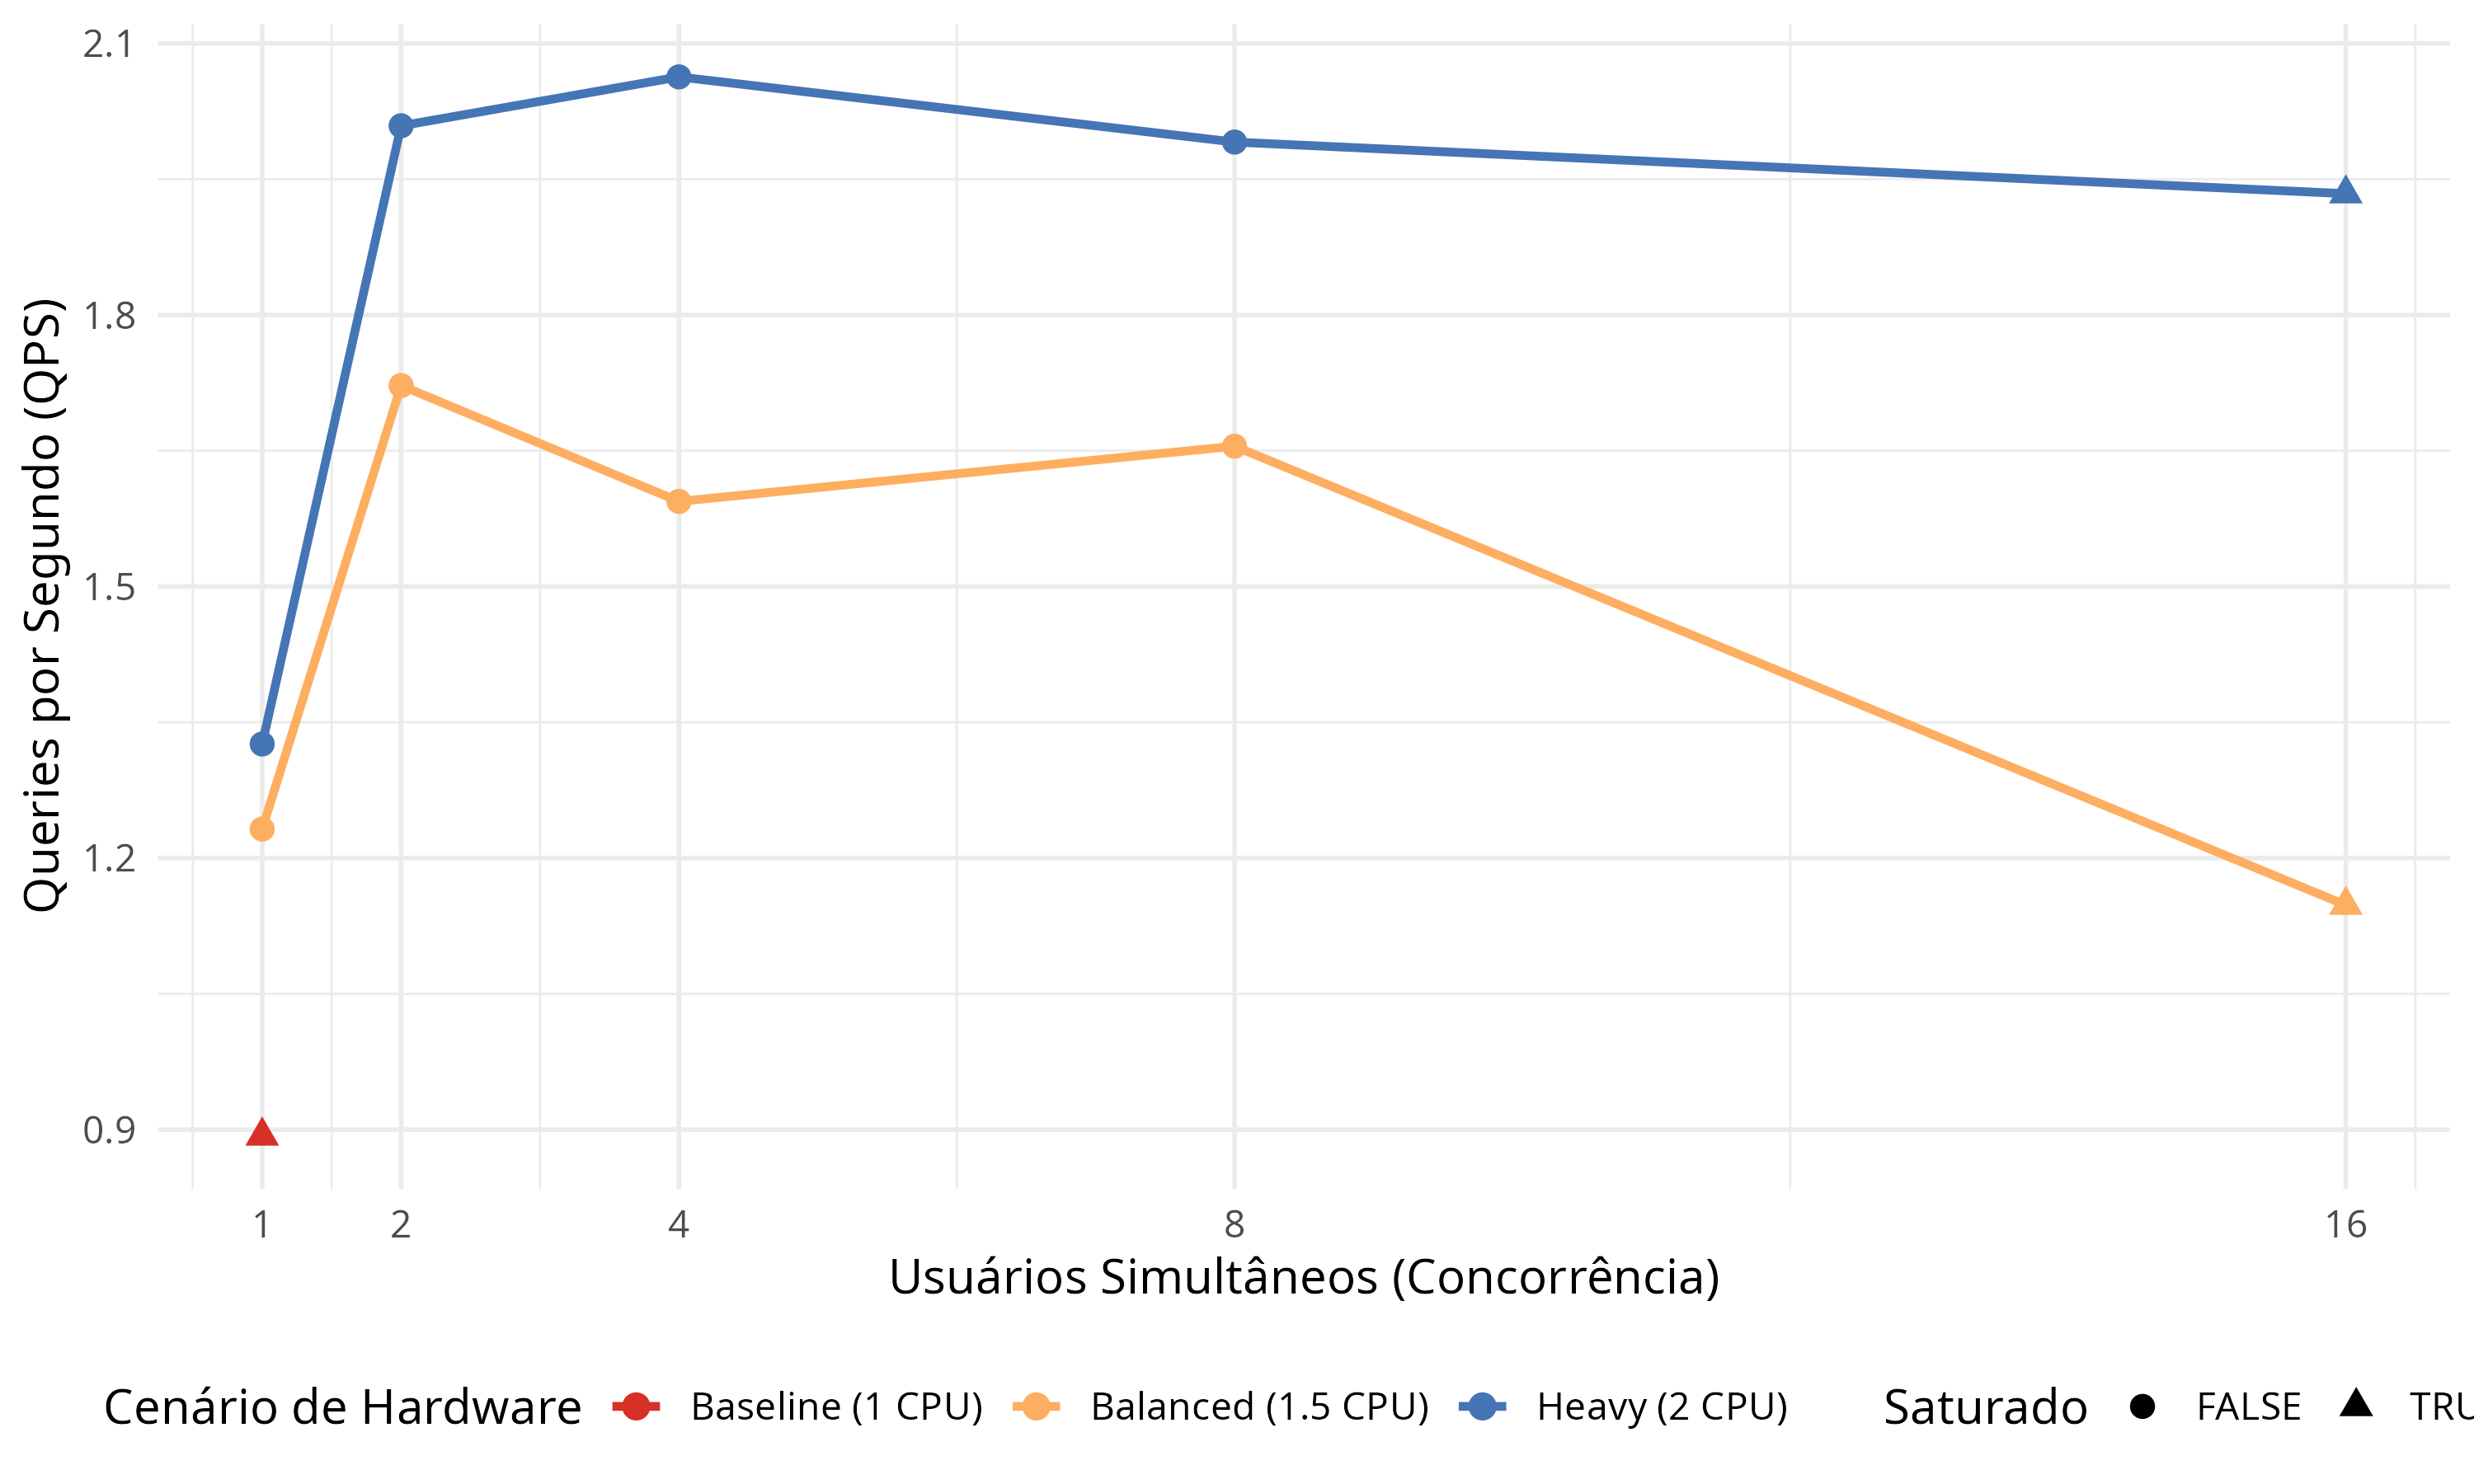
\includegraphics[width=0.8\textwidth]{images/qps_saturation.png}
    \caption{Curva de saturação: Limite de vazão da plataforma (QPS) por perfil de hardware.}
    \label{fig:qps_saturation}
\end{figure}

\begin{figure}[htpb]
    \centering
    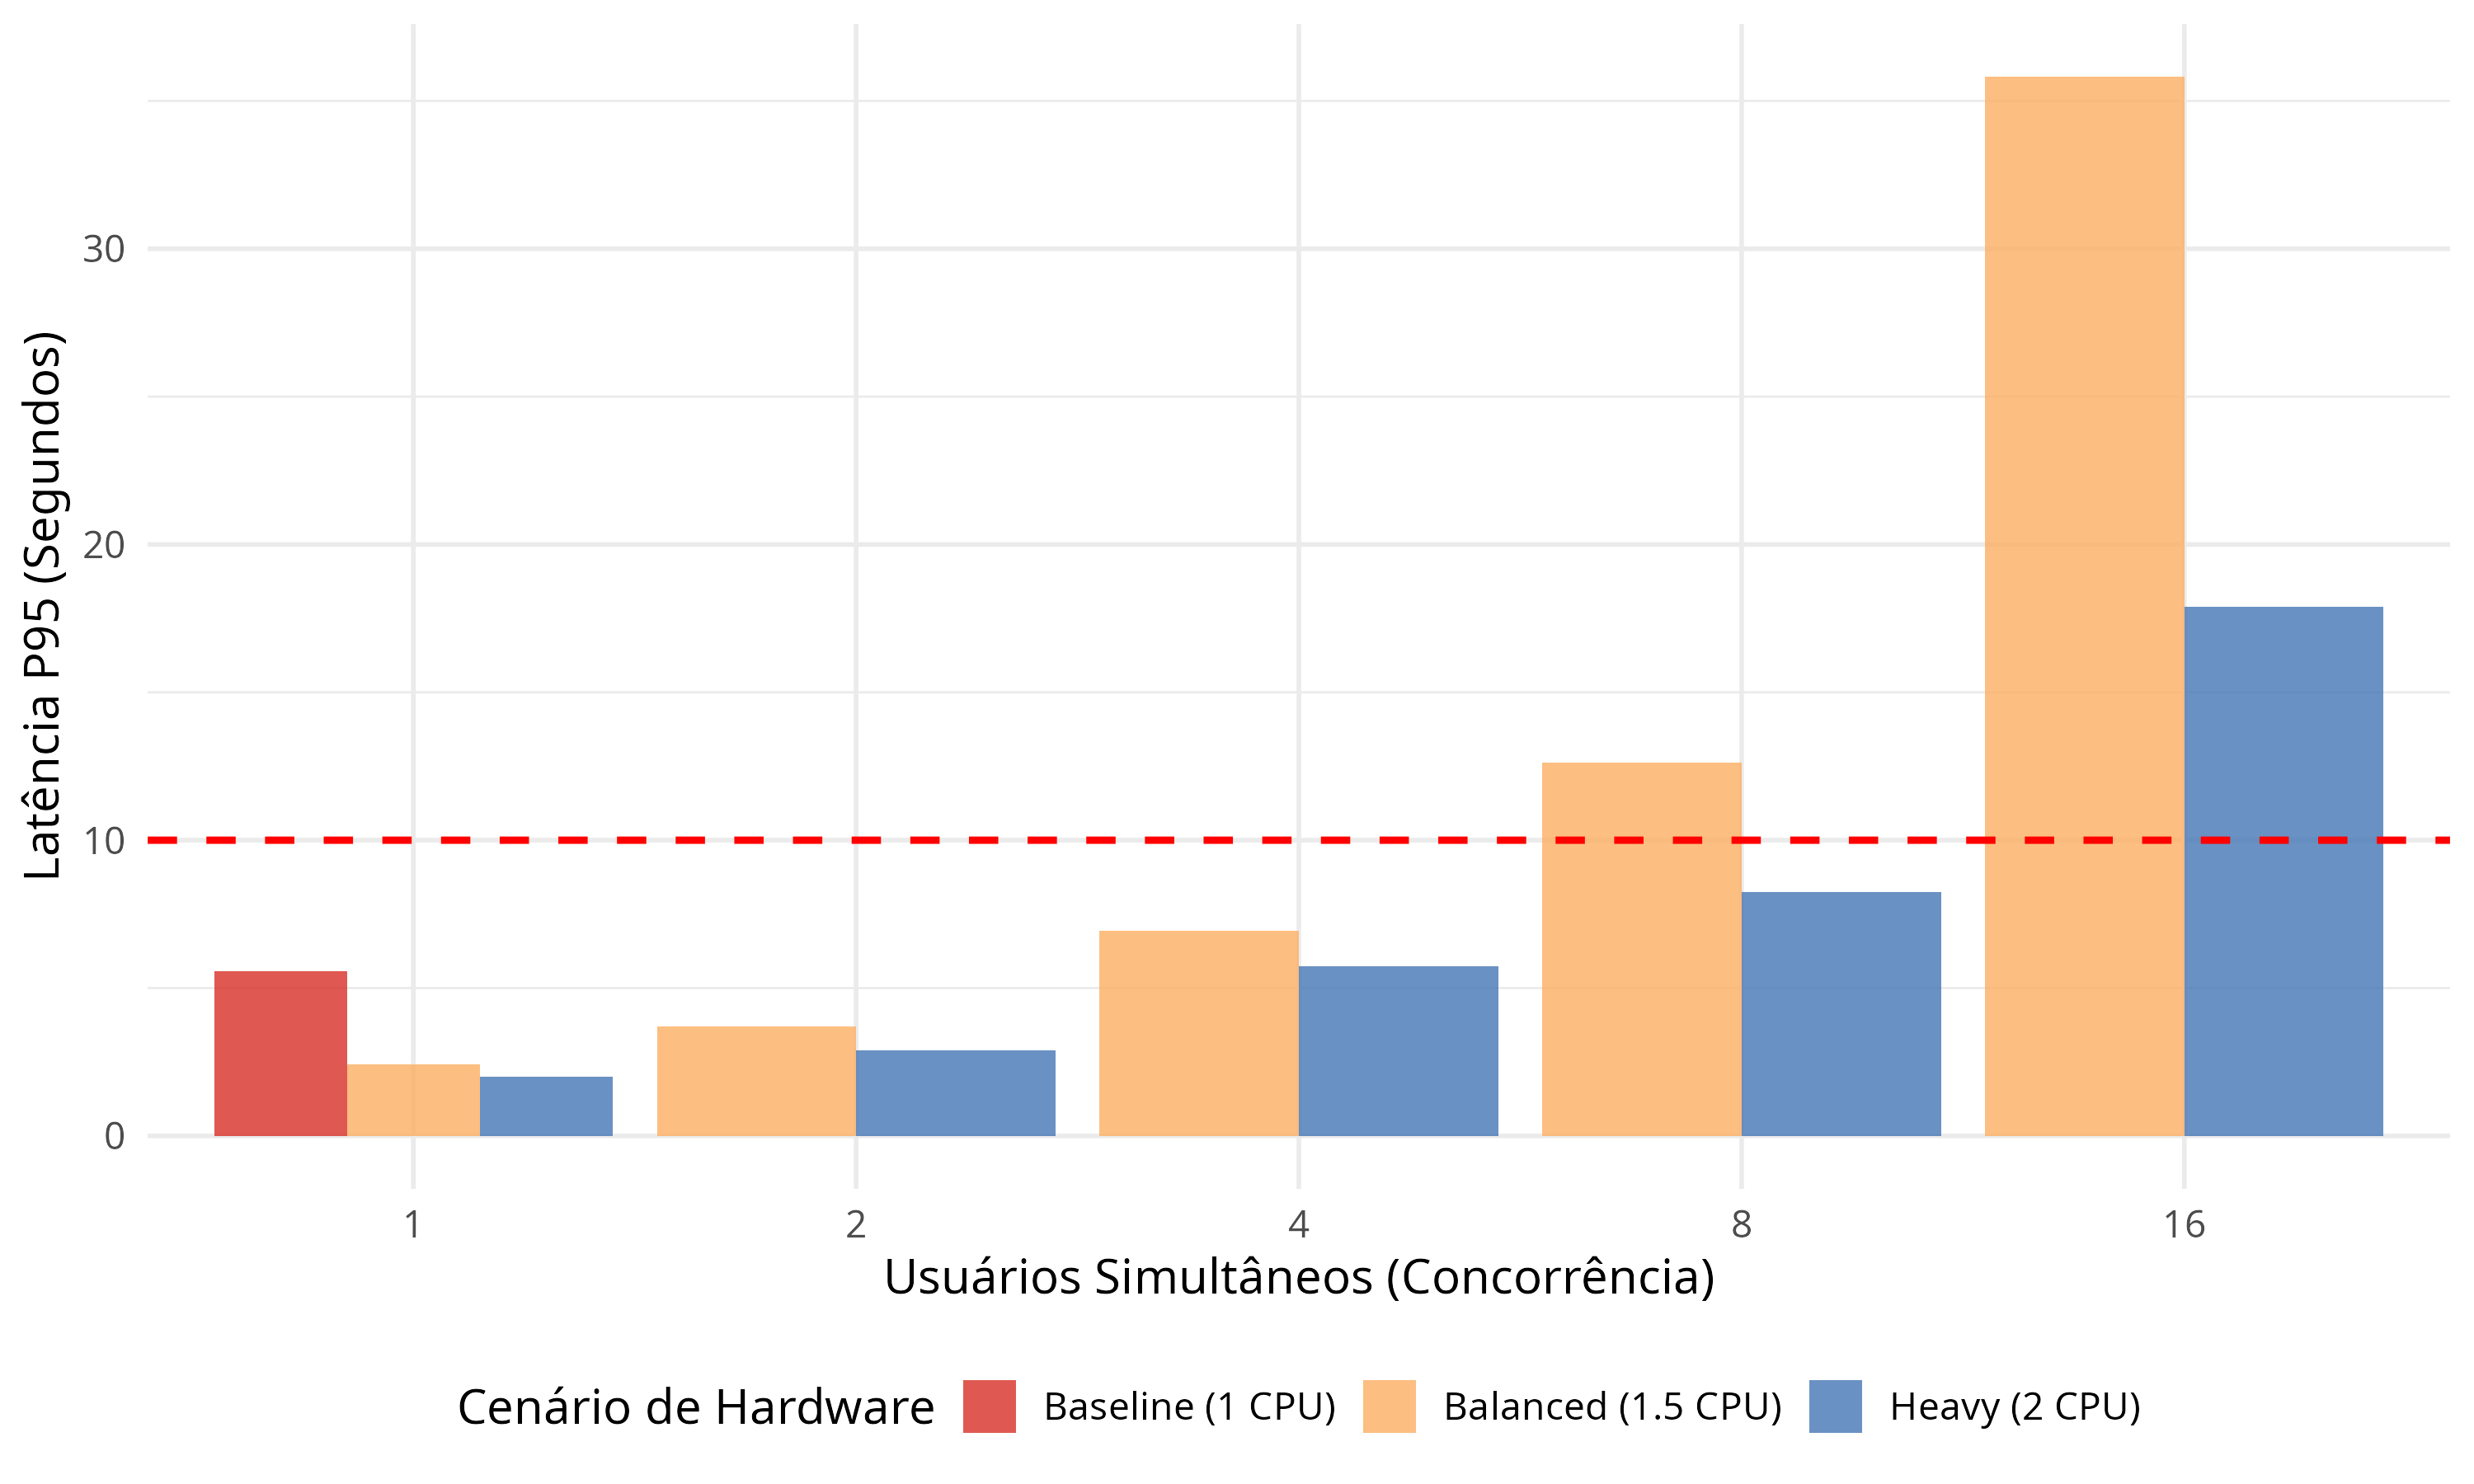
\includegraphics[width=0.8\textwidth]{images/p95_latency.png}
    \caption{Degradação da Latência P95 durante escalonamento exponencial de usuários.}
    \label{fig:p95_latency}
\end{figure}

\subsection{Eficiência do Mecanismo de Cache}

O uso do \textit{Broker Cache} no Druid acelerou varreduras completas e matrizes poligonais densas em até $40\%$. No cenário balanceado, uma extração fria (\textit{disco}) que levava $17,6s$ foi reduzida para $10,9s$ no cache (\textit{memória}). Contudo, em consultas extremamente simples (ex: \texttt{COUNT(*)} puro), o custo de rede para descriptografar a chave do cache gerou um levíssimo \textit{Overhead}, superando a velocidade da leitura nativa em colunas do disco.

\begin{figure}[htpb]
    \centering
    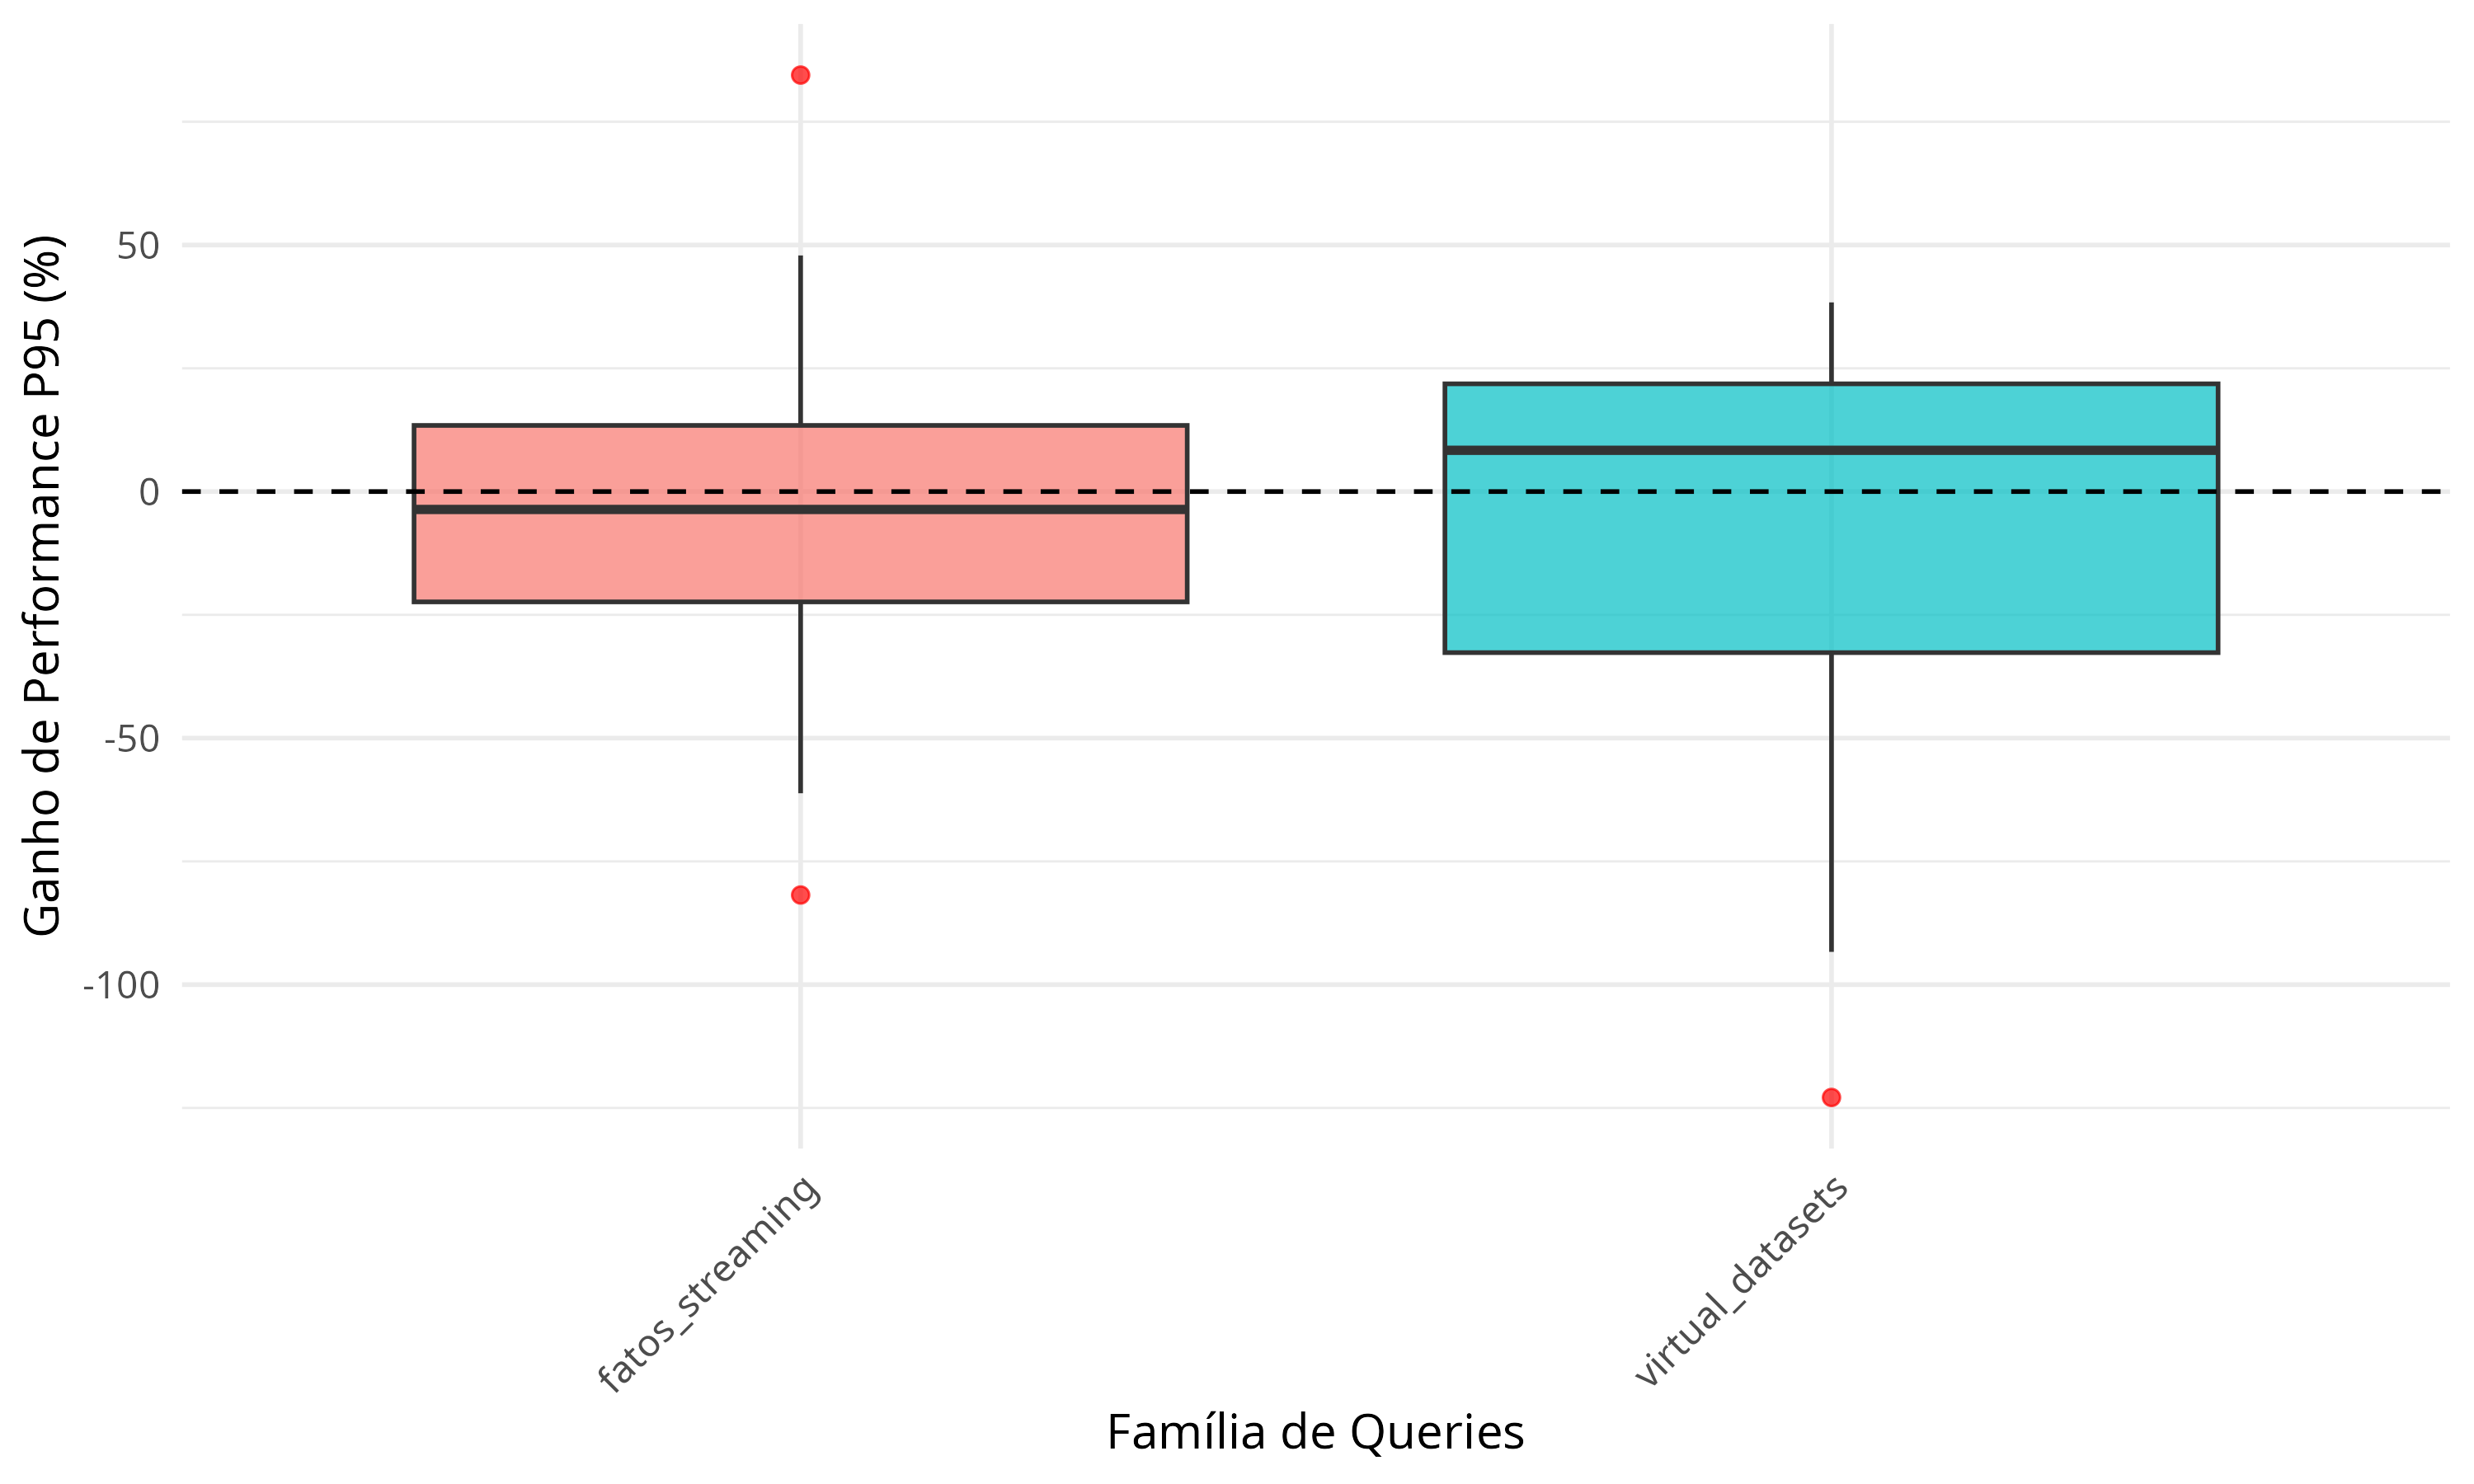
\includegraphics[width=0.8\textwidth]{images/cache_boxplot.png}
    \caption{Dispersão de ganhos obtidos entre leituras no disco (Cold) e em memória (Warm).}
    \label{fig:cache_efficiency}
\end{figure}

\subsection{Consumo Físico de Contêineres}

A análise nativa via Docker confirmou um rigoroso limite arquitetural de uso de memória. O consumo de RAM nos nós analíticos não ultrapassou $90\%$ sob as piores cargas, mantendo uma média de $75\%$. Sem episódios de troca em disco (\textit{Swap}) ou mortes lógicas (\textit{OOM Killed}), conclui-se que o gargalo restringe-se às vCPUs.

\begin{figure}[htpb]
    \centering
    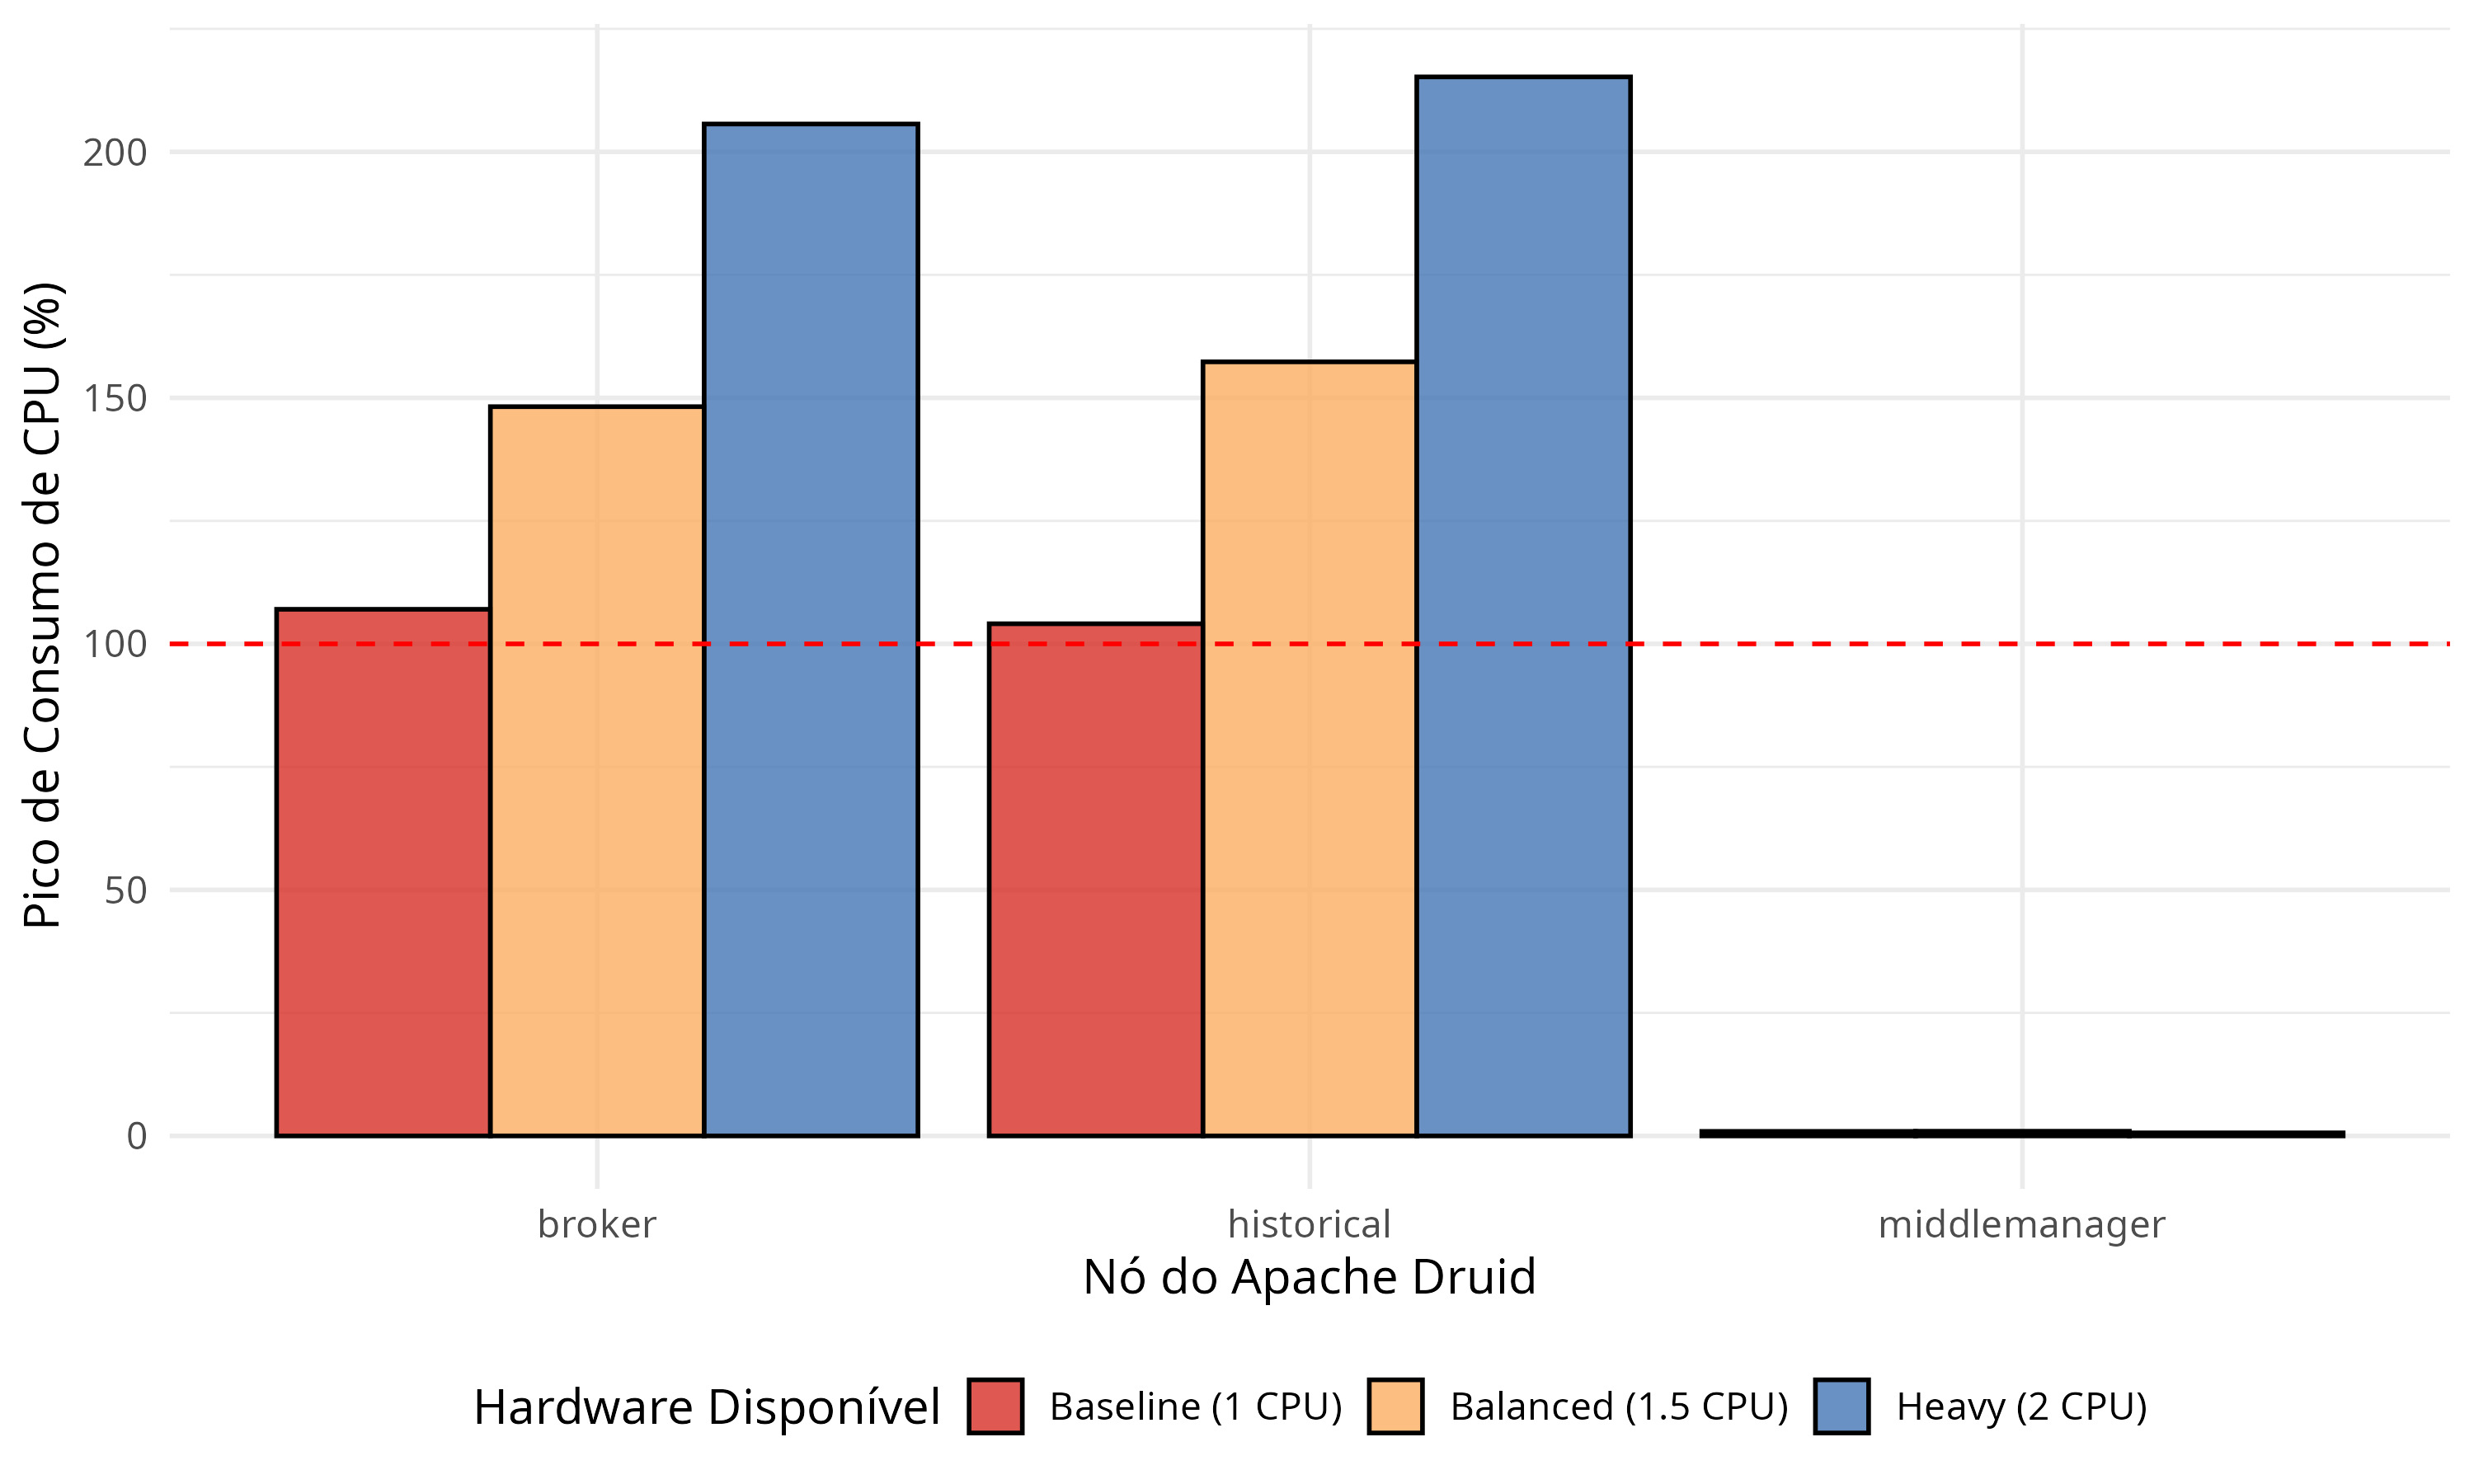
\includegraphics[width=0.8\textwidth]{images/cpu_peaks.png}
    \caption{Picos de estresse de CPU registrados por nó isolado do cluster.}
    \label{fig:cpu_peaks}
\end{figure}

\subsection{Hotspots: Gargalos Dimensionais e Armazenamento}

A consulta de maior custo foi o cruzamento espacial dinâmico, demandando longos 36 segundos sob hardware moderado. Fica provado que processar \textit{Joins} relacionais geoespaciais sob demanda limita o painel, exigindo que a desnormalização (\textit{ETL}) seja deslocada previamente para \textit{frameworks} otimizados, como o Apache Spark.

Em contrapartida à lentidão da junção analítica, a imensa vantagem do banco reflete-se na compressão extrema dos dados armazenados (Tabela~\ref{tab:storage_footprint}).

\begin{table}[htpb]
\centering
\caption{Pegada em disco consolidada das principais tabelas Fato e Dimensões.}
\label{tab:storage_footprint}
\begin{tabular}{lr}
\toprule
\textbf{Tabela (Datasource)} & \textbf{Tamanho Original (Druid)} \\
\midrule
Fato Focos (3.3M linhas) & 476 MB \\
Dimensões Terras Indígenas & 56 MB \\
Fato Eventos Clima & 34 MB \\
Outros Lookups & $\sim$1 MB \\
\midrule
\textbf{Total Compactado} & \textbf{566 MB} \\
\bottomrule
\end{tabular}
\end{table}

\section{Diagnóstico Arquitetural e Plano de Ação}

A exaustiva bateria de testes de estresse não apenas validou a robustez atual do sistema CCO-DataOps, como também elucidou precisamente onde e como ocorrem as fraturas de tempo de resposta. A capacidade de prever falhas possibilita traçar um plano de mitigação focado em decisões de infraestrutura e re-arquitetura lógica de dados.

\subsection{Onde o Sistema Trava? (Diagnóstico Final)}
Ficou inequivocamente comprovado que o engarrafamento de latência e de usabilidade aos analistas reside \textbf{quase inteiramente na exaustão das vCPUs do Apache Druid}. 

O Apache Superset atua como mero visualizador web. Quando dezenas de usuários clicam simultaneamente em painéis mistos de visualização (como os elaborados mapas térmicos de Focos de Incêndio justapostos a cruzamentos logísticos e indígenas), a requisição atinge a API do Druid. O Druid, por sua vez, colapsa seu motor de cálculos ao ser obrigado a aplicar ordenações complexas (\textit{TopN}) e cruzamentos dimensionais espaciais (\textit{Joins}) atrelados a monstruosas cordas de vértices poligonais em formato GeoJSON. Sendo a infraestrutura totalmente de perfil \textit{CPU-Bound}, o gargalo não provém de trocas de disco ou estouro de memória RAM, mas da fila de cálculos de rede do processador central tentando finalizar o cruzamento poligonal a tempo.

\subsection{Plano de Ação: O que pode ser aprimorado?}

A partir das evidências registradas em laboratório, delinearam-se três frentes de aprimoramentos para absorver um aumento exponencial na base de usuários de uma Central de Operações de Comando:

\begin{enumerate}
    \item \textbf{Recalibração Tática de Hardware (Verticalização Específica):}
    \begin{itemize}
        \item Uma vez extinto o "Mito da RAM" no Druid --- cuja utilização manteve-se constantemente reclusa aos limites médios de $75\%$ --- o capital de orçamentação \textit{Cloud} (seja em AWS EC2 ou Azure) deve ser exclusivamente vertido para a locação de mais processadores (vCPUs) direcionados às máquinas que operam os papéis de \textit{Broker} e \textit{Historical}. Evita-se, assim, desperdício financeiro alocando Memória estática que não impulsiona cruzamentos em tempo real.
    \end{itemize}

    \item \textbf{Achatamento Espacial e Desnormalização (Refatoração de ETL):}
    \begin{itemize}
        \item Os \textit{Joins} espaciais (especialmente a junção Fatos $\leftrightarrow$ Terras Indígenas) provaram-se o calcanhar de Aquiles computacional, atingindo inaceitáveis dezenas de segundos na resolução analítica.
        \item Como o Apache Druid prospera com estruturas planas (\textit{Flat Tables}), a solução arquitetural perene é migrar a responsabilidade deste cruzamento pesado para a etapa anterior da malha de dados. Utilizar o \textit{Apache Spark} (no \textit{Pipeline} ETL) para pré-calcular e engolir em definitivo o código IBGE, Siglas, Nomes e Etnologias para dentro da própria \texttt{fato\_focos\_incendio} (Desnormalização Absoluta), liquidando permanentemente o custo do \textit{Join} dinâmico espacial do painel interativo.
    \end{itemize}

    \item \textbf{Reestruturação Limitada dos Virtual Datasets:}
    \begin{itemize}
        \item O Custo de Operações dos Mapas no Superset ainda é fortemente amarrado aos limites de ordenação via código Jinja. Uma readequação materializando \textit{views} agregadas e compactadas diretamente dentro do armazenamento colunar (\textit{Rollup} avançado nas métricas geográficas) eliminaria as complexas lógicas de \texttt{GROUP BY} empurradas em tempo de visualização via API.
    \end{itemize}
\end{enumerate}

Em conclusão, a infraestrutura analítica do CCO-DataOps operou excepcionalmente bem até seu iminente \textit{trade-off}. As melhorias catalogadas não atestam falhas, mas norteiam a fase final de maturidade de Produto de Dados rumo ao escalonamento ilimitado.

\section{Considerações Finais}

A implementação e subsequente estresse da arquitetura analítica do CCO-DataOps consolidam a eficácia das modernas engrenagens de \textit{DataOps} na gestão de crises ambientais e infraestrutura de missão crítica. Através do acoplamento do Apache Superset ao motor OLAP do Apache Druid, demonstrou-se, com respaldo em metodologias laboratoriais, a viabilidade técnica de extrair \textit{insights} imediatos do cruzamento de bilhões de dados telemétricos geoespaciais com dicionários complexos do território brasileiro.

O arcabouço tecnológico provou ser resiliente e perfeitamente contido no espectro de custos de computação em nuvem moderada. Evidenciou-se que a adoção precoce de compactação profunda (\textit{Storage Footprint} otimizado) e varreduras colunares anula a necessidade de dispêndios orçamentários volumosos em armazenamento. Além disso, as descobertas obtidas pelo isolamento das anomalias de \textit{performance} fornecem aos Engenheiros de Dados do projeto diretrizes clarividentes --- como a imperiosa migração de \textit{Joins} onerosos para etapas puras de \textit{ETL} via Apache Spark.

Em última instância, este relatório atesta não somente a capacidade atual da plataforma de operar em cenários limítrofes, mas, fundamentalmente, firma o alicerce científico e arquitetural necessário para escalar o monitoramento de Focos de Incêndio a níveis governamentais absolutos, unindo dados abertos de saúde, logística e segurança à fronteira da visualização analítica geoespacial.


\end{document}
